\section{Presentation Logic Layer}

%What pages will be present in your project? briefly indicate how your web site will be organized
In our Car Rental web application's Presentation Logic Layer, we've crafted intuitive pages to streamline user interaction:\\

\begin{itemize}
    \item The Registration Page allows swift account creation.
    \item The Add Cars Page simplifies fleet management.
    \item The User Dashboard offers personalized account insights.
    \item My Rental Cars Page facilitates document uploads.
    \item The Car Information Page provides detailed rental insights.
    \item The Home Page serves as a user-friendly entry point.\\
\end{itemize}

This setup ensures a seamless user experience and efficient navigation throughout the platform.

\subsection{Home Page}

%For the main pages put a mockup and describe it in detail.

\begin{figure}[h]
\centering
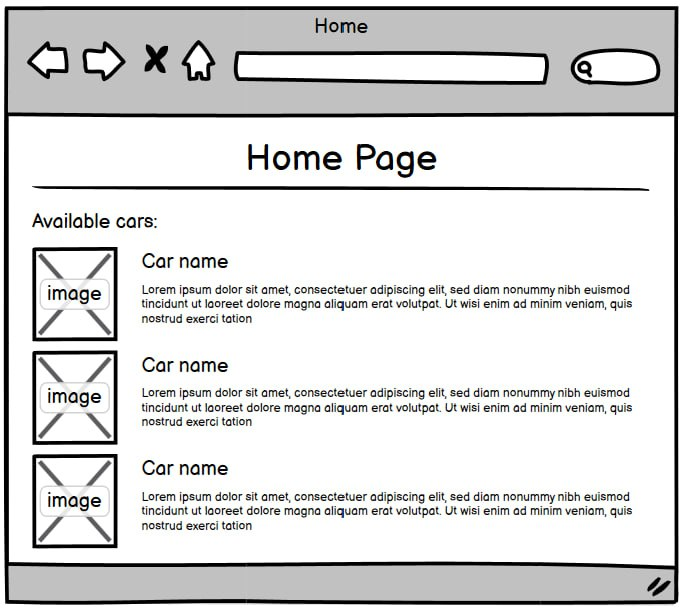
\includegraphics[width=0.7\textwidth, inner]{sections/HomePage.jpg}
\caption{Home Page}
\end{figure}\\
The Home Page serves as the main entry point, welcoming users with an overview of available cars, promotions, and featured vehicles. It provides a search and browsing interface, user sign-in options, customer testimonials, and informational resources to guide users seamlessly through the platform.\newpage
 \subsection{Registration Page: }

%For the main pages put a mockup and describe it in detail.

\begin{figure}[h]
\centering
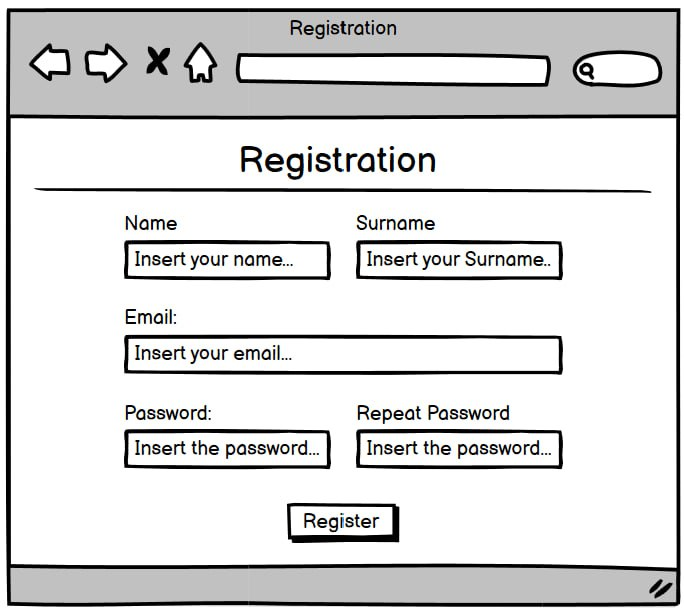
\includegraphics[width=0.7\textwidth, inner]{sections/Registration.jpg}
\caption{Registration Page}
\end{figure}\\

The Registration Page allows new users to create accounts by providing essential information such as their name, email address, password, and contact details. The registration form is user-friendly and intuitive, guiding users through the process step by step. Once the form is submitted, the user's account is created, and they gain access to personalized features and functionalities within the application. The Registration Page may also include optional fields for users to provide additional information, such as their preferences or interests, to tailor their experience further. Robust validation ensures that all entered data is accurate and secure, protecting user privacy and preventing fraudulent.\newpage
 \subsection{Add Cars Page: }

%For the main pages put a mockup and describe it in detail.

\begin{figure}[h]
\centering
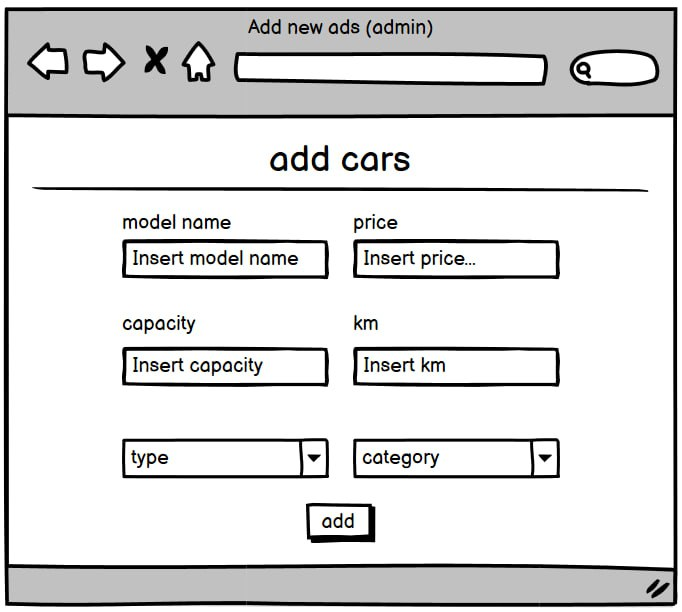
\includegraphics[width=0.7\textwidth, inner]{sections/AddCars.jpg}
\caption{Add Cars Page}
\end{figure}\\

The Add Cars Page is accessible to administrators or authorized users responsible for managing the rental fleet. It features a comprehensive form where users can input detailed information about new cars to be added to the inventory. The form includes fields for the car's license plate number, rental rate, capacity, model name, category, current status, brand name, and any additional specifications or features. Users can upload photos of the car to provide visual representations for potential renters. Once the form is submitted, the new car is added to the rental inventory, and its details are updated in the database. The Add Cars Page streamlines the process of adding new vehicles, ensuring that the rental fleet remains up-to-date and well-maintained.\newpage
 \subsection{User Dashboard:  }

%For the main pages put a mockup and describe it in detail.

\begin{figure}[h]
\centering
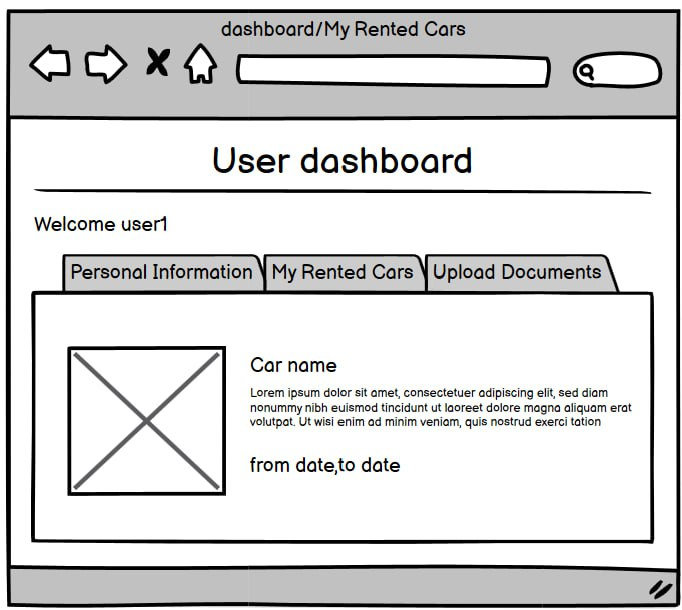
\includegraphics[width=0.7\textwidth, inner]{sections/UserDashboard.jpg}
\caption{User Dashboard Page}
\end{figure}\\


The User Dashboard serves as a centralized hub where registered users can access and manage their account information. It provides a personalized view of the user's profile, including their name, contact details, rental history, and preferences. Users can easily update their profile information, such as changing their password or updating their contact information, directly from the dashboard. The dashboard also displays any ongoing rental transactions, including the dates, duration, and status of each rental. Users can track their rental history, view past transactions, and access digital copies of rental agreements or receipts. The User Dashboard enhances user engagement and satisfaction by providing a convenient and intuitive interface for managing account activities and rental-related tasks.\newpage
 \subsection{Car Information Page:  }

%For the main pages put a mockup and describe it in detail.

\begin{figure}[h]
\centering
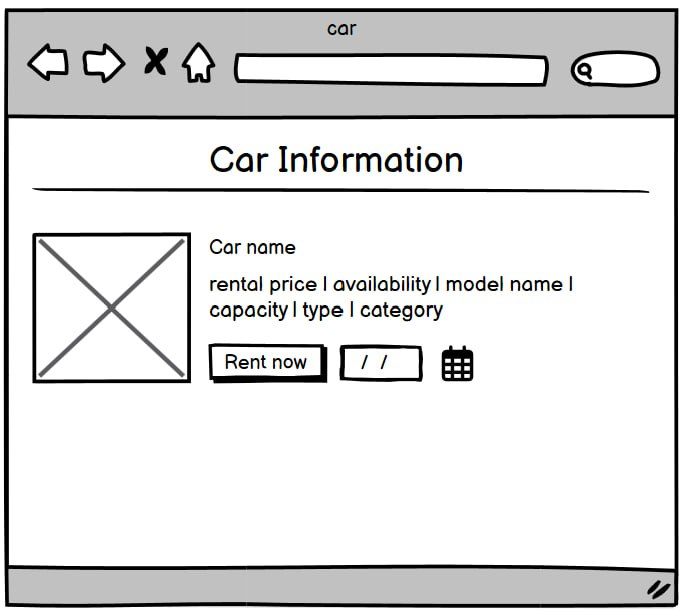
\includegraphics[width=0.7\textwidth, inner]{sections/CarInformation.jpg}
\caption{Car Information Page}
\end{figure}\\
The Car Information Page provides detailed insights into individual cars available for rental. It features comprehensive information about each car, including specifications, features, rental history, and associated fees. Users can view high-quality photos of the car from different angles to get a better understanding of its appearance and condition. The page includes detailed descriptions of the car's make, model, year, mileage, and any special features or amenities it may have. Users can also see the availability of the car for their desired rental dates and check the rental rates and fees associated with renting the car. Clear call-to-action buttons prompt users to initiate the rental process, such as requesting a reservation or contacting customer support for assistance. The Car Information Page helps users make informed decisions about their rental choices by providing comprehensive and detailed information about each car in the rental inventory.\newpage

 
 
 
 
 